\chapter{Methods}
\label{ch:Methods}
In this chapter various methods using different sensors to estimate the car's pitch angle and thus the ramp angle, as well as other properties of the ramp, such as the width and length, will be described.
The problem definition is discussed in \cref{sec:road_grade_definition}.
Before being able to use the sensor measurements, a coordinate frame transformation to the device frame is necessary.
This problem is described in \cref{sec:coordinate_frames}.
In \cref{sec:methods_imu} multiple methods to estimate the car's pitch angle using an \gls{imu} are described.
The angle is then used to identify a ramp.
A novel method using a \gls{lidar} sensor will be represented in \cref{sec:methods_lidar}.
It tracks the distance to the ramp and estimates the angle and width of the ramp.
Finally, a ramp detection algorithm using a camera and a trained neural network will be presented.


\section{Road grade definition}
\label{sec:road_grade_definition}
\begin{figure}[htb]
	\centering
	\documentclass[11pt]{standalone}
\usepackage{tikz}
\usetikzlibrary{angles, calc, decorations.pathmorphing, quotes, spy}

\begin{document}
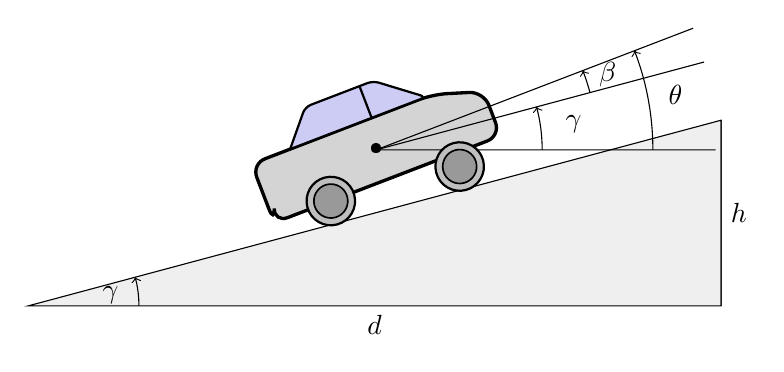
\begin{tikzpicture}[scale=.88]
    % Define/Calc ramp parameters
    % Ramp length
    \def\rl{10};
    % Ramp angle [deg]
    \def\ra{15};
    % Ramp height
    \def\rh{{tan(\ra)*\rl}};

    % RAMP
    % Define the points
    \coordinate (A) at (0,0);
    \coordinate (B) at ($(A) + (\rl,0)$);
    \coordinate (C) at ($(B) + (0,\rh)$);
    % Draw and fill ramp
    \filldraw[draw=black, fill=lightgray!25] (A) -- (B) -- (C) -- cycle;
    % Label length and draw angle
    \path (A) -- (B) node [midway, below] {$d$}
    pic[draw, ->, angle radius=40pt,
            angle eccentricity=0.75, "$\gamma$"]{angle=B--A--C};
    % Label height
    \draw (B) -- (C) node [midway, right] {$h$};

    % CAR
    % Tilt whole car
    \begin{scope}[scale=0.7, xshift=\rl*0.5 cm, yshift=1.9 cm, rotate=\ra]

        % Car height
        \def\ch{2}
        % Car length
        \def\cl{5}
        % Car body height
        \def\bh{\ch*0.65}
        % Roof length
        \def\rl{\cl*0.6}
        % Roof height
        \def\rh{\ch*0.35}
        % Car tilt angle
        \def\ct{6}

        % Tilt body without wheels
        \begin{scope}[rotate=\ct, yshift=-0.2cm]
            % Anchor point is southwest
            \coordinate (b) at (0,0);
            % Offset to roof and wheels
            \coordinate (r) at ($(b) +(\cl*0.17,\ch*0.65)$);
            \coordinate (w) at ($(b) + (\cl*0.25,0)$);
            % Body
            \draw[black, fill=black!17, rounded corners=1.2ex, very thick]
            (b) -- ++(0,\bh) -- ++(\cl*1/5,0) --  ++(\cl*3/5,0) -- ++(\cl*1/5,-\bh*0.25)
            -- ++(0, -\bh*0.75) -- (b) -- cycle;
            % Roof
            \draw[very thick, rounded corners=0.5ex, fill=black!20!blue!20!white,thick]
            (r) -- ++(0.2*\rl,\rh) -- ++(0.5*\rl,0) -- ++(0.3*\rl,-\rh) -- (r);
            \draw[thick] (r)++(\rl*0.6,0) -- ++(0,\rh);

            % Car middle point
            \coordinate (m) at (\cl*0.5, \bh*0.5);
            \node at (m) {\textbullet};
            % Line parallel to body
            \draw (m) -- ++(7,0) coordinate (pb);
            % Line parallel to ramp
            \draw[rotate = -\ct] (m) -- ++(7,0) coordinate (pr);
            % Line parallel to ground
            \draw[rotate = -\ct-\ra] (m) -- ++(7,0) coordinate (pg);
            % Draw angles
            \path (pb) -- (pr)
            pic[draw, ->, angle radius=60pt, angle eccentricity=1.2, "$\gamma$"] {angle = pg--m--pr}
            pic[draw, ->, angle radius=80pt, angle eccentricity=1.1, "$\beta$"] {angle = pr--m--pb}
            pic[draw, ->, angle radius=100pt, angle eccentricity=1.1, "$\theta$"] {angle = pg--m--pb};
        \end{scope}

        % Wheels
        \draw[draw=black,fill=gray!50,thick] (w) circle (.5);
        \draw[draw=black,fill=gray!50,thick] (w) ++(\cl*0.55,0) circle (.5);
        % Inner wheels
        \draw[draw=black,fill=gray!80,semithick] (w) circle (.35);
        \draw[draw=black,fill=gray!80,semithick] (w) ++(\cl*0.55,0) circle (.35);
    \end{scope}
\end{tikzpicture}
\end{document}
	\caption[Ramp angle definition]{Car driving on a ramp. Due to forward acceleration the car tilts back.}
	\label{fig:tikz_car_tilt}
\end{figure}
The road grade $\alpha$ is the angle between the road plane and the ground plane.
The ground plane is perpendicular to the gravity vector.
The road grade can be represented as an angle
\begin{equation}
	\alpha = \arctan(\frac{h}{d})
\end{equation}
or in percentage
\begin{equation}
	r = 100\cdot\tan(\alpha).
\end{equation}
The pitch angle $\theta$ of the car is defined as the angle between the ground plane and the longitudinal axis of the car.
If the car accelerates or decelerates the suspension does get compressed in the back or respectively front, which makes the pitch angle not in alignment with the road grade anymore.
The difference between the two angles is defined as $\beta = \theta - \alpha$ and may also occur due to rotational movement or vibrations.
The mentioned variables are visualized in \cref{fig:tikz_car_tilt}.



\section{Coordinate frames}
\label{sec:coordinate_frames}
A common problem is that the coordinate frames of the sensors are usually not aligned with the device (in this case the car) frame, see \cref{fig:tikz_car_frames}.
To get meaningful results, the sensor frames must first be aligned with the car frame.
Semi-automatic calibration methods for the \gls{imu} and \gls{lidar} sensor will be represented in \cref{ssec:calibration_imu} and \cref{ssec:calibration_lidar} respectively, which determine the necessary rotation to align both frames.
But the translation difference between the coordinate frames can not be easily estimated or requires a more sophisticated calibration setup which was not available, and must be measured by hand.\\
The coordinate frame of the car has the x-axis pointing in the direction of travel , the y-axis to the left and the z-axis upwards.
The center of the coordinate system of the car is located at the center in the front of the car at the height of the wheel axle.
\begin{figure}[htb]
	\centering
	\documentclass{standalone}
\usepackage{tikz}
\usetikzlibrary{angles, calc, decorations.pathmorphing, quotes, spy}

\begin{document}
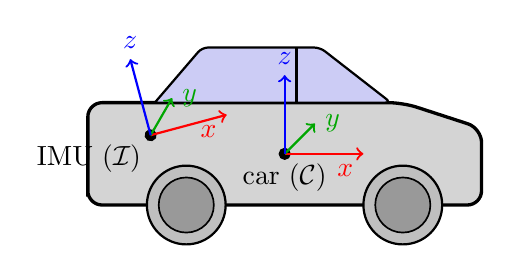
\begin{tikzpicture}[scale=1]
    % Define car parameters
    % Car height
    \def\ch{2}
    % Car length
    \def\cl{5}
    % Car body height
    \def\bh{\ch*0.65}
    % Roof length
    \def\rl{\cl*0.6}
    % Roof height
    \def\rh{\ch*0.35}
    % Car tilt angle
    \def\ct{6}
    % Anchor point is southwest
    \coordinate (b) at (0,0);
    % Offset to roof and wheels
    \coordinate (r) at ($(b) +(\cl*0.17,\ch*0.65)$);
    \coordinate (w) at ($(b) + (\cl*0.25,0)$);

    % Body
    \draw[black, fill=black!17, rounded corners=1.2ex, very thick]
    (b) -- ++(0,\bh) -- ++(\cl*1/5,0) --  ++(\cl*3/5,0) -- ++(\cl*1/5,-\bh*0.25)
    -- ++(0, -\bh*0.75) -- (b) -- cycle;
    % Roof
    \draw[very thick, rounded corners=0.5ex, fill=black!20!blue!20!white,thick]
    (r) -- ++(0.2*\rl,\rh) -- ++(0.5*\rl,0) -- ++(0.3*\rl,-\rh) -- (r);
    % \draw[thick] ($(r) + (\cl*0.5,\bh)$) -- ++(0,\rh);
    \draw[thick] (r)++(\rl*0.6,0) -- ++(0,\rh);

    % Wheels
    \draw[draw=black,fill=gray!50,thick] (w) circle (.5);
    \draw[draw=black,fill=gray!50,thick] (w) ++(\cl*0.55,0) circle (.5);
    % Inner wheels
    \draw[draw=black,fill=gray!80,semithick] (w) circle (.35);
    \draw[draw=black,fill=gray!80,semithick] (w) ++(\cl*0.55,0) circle (.35);

    % Car middle point
    \coordinate (m) at (\cl*0.5, \bh*0.5);
    \filldraw (m) circle (2pt) node[below] {car ($\mathcal{C}$)};
    % Coordinate frames
    \draw[thick,->, red] (m) -- ++(1,0,0) node[anchor=north east]{$x$};
    \draw[thick,->, black!35!green] (m) -- ++(0,0,-1) node[anchor=west]{$y$};
    \draw[thick,->, blue] (m) -- ++(0,1,0) node[anchor=south]{$z$};

    % IMU middle point (random)
    \begin{scope}[rotate=15]
        \coordinate (mi) at (\cl*0.2, \bh*0.5);
        \filldraw (mi) circle (2pt) node[below left] {IMU ($\mathcal{I}$)};
        % Coordinate frames
        \draw[thick,->, red] (mi) -- ++(1,0,0) node[anchor=north east]{$x$};
        \draw[thick,->, black!35!green] (mi) -- ++(0,0,-1) node[anchor=west]{$y$};
        \draw[thick,->, blue] (mi) -- ++(0,1,0) node[anchor=south]{$z$};
    \end{scope}
\end{tikzpicture}
\end{document}
	\caption[Sensor coordinate frames]{Example of a typical sensor setup. All measurements of the sensors must be transformed, such that they align with the car frame.}
	\label{fig:tikz_car_frames}
\end{figure}



\section{\glsentryshort{imu}}
\label{sec:methods_imu}
Before being able to apply the different methods, a transformation from the sensor frame to the car frame is necessary.
This is described in \cref{ssec:calibration_imu}.
After the transformation an estimation of the car's pitch angle is possible, for which different methods are presented in \cref{ssec:road_grade_estimation}.
In \cref{ssec:ramp_detection_imu} a ramp detection algorithm based on the estimated pitch angle is presented.
Furthermore, a method to estimate the average ramp angle and length of the ramp is proposed.


\subsection{Calibration}
\label{ssec:calibration_imu}
\begin{figure}[htb]
	\centering
	\begin{subfigure}[b]{0.3\textwidth}
		\centering
		\documentclass[11pt]{standalone}
\usepackage{tikz}

\newcommand{\rotateRPY}[3]% roll, pitch, yaw
{   \pgfmathsetmacro{\rollangle}{#1}
    \pgfmathsetmacro{\pitchangle}{#2}
    \pgfmathsetmacro{\yawangle}{#3}

    % to what vector is the x unit vector transformed, and which 2D vector is this?
    \pgfmathsetmacro{\newxx}{cos(\yawangle)*cos(\pitchangle)}
    \pgfmathsetmacro{\newxy}{sin(\yawangle)*cos(\pitchangle)}
    \pgfmathsetmacro{\newxz}{-sin(\pitchangle)}
    \path (\newxx,\newxy,\newxz);
    \pgfgetlastxy{\nxx}{\nxy};

    % to what vector is the y unit vector transformed, and which 2D vector is this?
    \pgfmathsetmacro{\newyx}{cos(\yawangle)*sin(\pitchangle)*sin(\rollangle)-sin(\yawangle)*cos(\rollangle)}
    \pgfmathsetmacro{\newyy}{sin(\yawangle)*sin(\pitchangle)*sin(\rollangle)+ cos(\yawangle)*cos(\rollangle)}
    \pgfmathsetmacro{\newyz}{cos(\pitchangle)*sin(\rollangle)}
    \path (\newyx,\newyy,\newyz);
    \pgfgetlastxy{\nyx}{\nyy};

    % to what vector is the z unit vector transformed, and which 2D vector is this?
    \pgfmathsetmacro{\newzx}{cos(\yawangle)*sin(\pitchangle)*cos(\rollangle)+ sin(\yawangle)*sin(\rollangle)}
    \pgfmathsetmacro{\newzy}{sin(\yawangle)*sin(\pitchangle)*cos(\rollangle)-cos(\yawangle)*sin(\rollangle)}
    \pgfmathsetmacro{\newzz}{cos(\pitchangle)*cos(\rollangle)}
    \path (\newzx,\newzy,\newzz);
    \pgfgetlastxy{\nzx}{\nzy};
}
\tikzset{RPY/.style={x={(\nxx,\nxy)},y={(\nyx,\nyy)},z={(\nzx,\nzy)}}}
% NOTE: I changed y and z axes, so it is now RYP instead of RPY

\begin{document}
\begin{tikzpicture}
    \draw[-latex] node at (3.5,0,0) {x} (0,0,0) -- (3,0,0);
    \draw[-latex] node at (0,0,-3.5) {y} (0,0,0) -- (0,0,-3);
    \draw[-latex] node at (0,3.5,0) {z} (0,0,0) -- (0,3,0);

    \rotateRPY{5}{5}{20}
    \begin{scope}[draw=red, text=red,fill=red,densely dashed,RPY]
        \draw[-latex] node at (3.5,0,0) {x} (0,0,0) -- (3,0,0);
        \draw[-latex] node at (0,0,-3.5) {y} (0,0,0) -- (0,0,-3);
        \draw[-latex] node at (0,3.5,0) {z} (0,0,0) -- (0,3,0);
    \end{scope}
    % \node[fill=white,fill opacity=0.7,text opacity=1] {RPY: $r$,$p$,$y$};
\end{tikzpicture}
\end{document}
		\caption{No axes are aligned}
		\label{fig:tikz_frame_transformation_init}
	\end{subfigure}
	\hfill
	\begin{subfigure}[b]{0.3\textwidth}
		\centering
		\documentclass[11pt]{standalone}
\usepackage{tikz}

\newcommand{\rotateRPY}[3]% roll, pitch, yaw
{   \pgfmathsetmacro{\rollangle}{#1}
    \pgfmathsetmacro{\pitchangle}{#2}
    \pgfmathsetmacro{\yawangle}{#3}

    % to what vector is the x unit vector transformed, and which 2D vector is this?
    \pgfmathsetmacro{\newxx}{cos(\yawangle)*cos(\pitchangle)}
    \pgfmathsetmacro{\newxy}{sin(\yawangle)*cos(\pitchangle)}
    \pgfmathsetmacro{\newxz}{-sin(\pitchangle)}
    \path (\newxx,\newxy,\newxz);
    \pgfgetlastxy{\nxx}{\nxy};

    % to what vector is the y unit vector transformed, and which 2D vector is this?
    \pgfmathsetmacro{\newyx}{cos(\yawangle)*sin(\pitchangle)*sin(\rollangle)-sin(\yawangle)*cos(\rollangle)}
    \pgfmathsetmacro{\newyy}{sin(\yawangle)*sin(\pitchangle)*sin(\rollangle)+ cos(\yawangle)*cos(\rollangle)}
    \pgfmathsetmacro{\newyz}{cos(\pitchangle)*sin(\rollangle)}
    \path (\newyx,\newyy,\newyz);
    \pgfgetlastxy{\nyx}{\nyy};

    % to what vector is the z unit vector transformed, and which 2D vector is this?
    \pgfmathsetmacro{\newzx}{cos(\yawangle)*sin(\pitchangle)*cos(\rollangle)+ sin(\yawangle)*sin(\rollangle)}
    \pgfmathsetmacro{\newzy}{sin(\yawangle)*sin(\pitchangle)*cos(\rollangle)-cos(\yawangle)*sin(\rollangle)}
    \pgfmathsetmacro{\newzz}{cos(\pitchangle)*cos(\rollangle)}
    \path (\newzx,\newzy,\newzz);
    \pgfgetlastxy{\nzx}{\nzy};
}
\tikzset{RPY/.style={x={(\nxx,\nxy)},y={(\nyx,\nyy)},z={(\nzx,\nzy)}}}
% NOTE: I changed y and z axes, so it is now RYP instead of RPY

\begin{document}
\begin{tikzpicture}
    \draw[-latex] node at (3.5,0,0) {x} (0,0,0) -- (3,0,0);
    \draw[-latex] node at (0,0,-3.5) {y} (0,0,0) -- (0,0,-3);
    \draw[-latex] node at (0,3.5,0) {z} (0,0,0) -- (0,3,0);

    \rotateRPY{0}{5}{0}
    \begin{scope}[draw=blue, text=blue,fill=blue,densely dashed,RPY]
        \draw[-latex] node at (3.5,0,0) {x} (0,0,0) -- (3,0,0);
        \draw[-latex] node at (0,0,-3.5) {y} (0,0,0) -- (0,0,-3);
        \draw[-latex] node at (0,3.5,0) {z} (0,0,0) -- (0,3,0);
    \end{scope}
    % \node[fill=white,fill opacity=0.7,text opacity=1] {RPY: 0,0,$y$};
\end{tikzpicture}
\end{document}
		\caption{Z axes are aligned}
		\label{fig:tikz_frame_transformation_intermediate}
	\end{subfigure}
	\hfill
	\begin{subfigure}[b]{0.3\textwidth}
		\centering
		\documentclass[11pt]{standalone}
\usepackage{tikz}

\newcommand{\rotateRPY}[3]% roll, pitch, yaw
{   \pgfmathsetmacro{\rollangle}{#1}
    \pgfmathsetmacro{\pitchangle}{#2}
    \pgfmathsetmacro{\yawangle}{#3}

    % to what vector is the x unit vector transformed, and which 2D vector is this?
    \pgfmathsetmacro{\newxx}{cos(\yawangle)*cos(\pitchangle)}
    \pgfmathsetmacro{\newxy}{sin(\yawangle)*cos(\pitchangle)}
    \pgfmathsetmacro{\newxz}{-sin(\pitchangle)}
    \path (\newxx,\newxy,\newxz);
    \pgfgetlastxy{\nxx}{\nxy};

    % to what vector is the y unit vector transformed, and which 2D vector is this?
    \pgfmathsetmacro{\newyx}{cos(\yawangle)*sin(\pitchangle)*sin(\rollangle)-sin(\yawangle)*cos(\rollangle)}
    \pgfmathsetmacro{\newyy}{sin(\yawangle)*sin(\pitchangle)*sin(\rollangle)+ cos(\yawangle)*cos(\rollangle)}
    \pgfmathsetmacro{\newyz}{cos(\pitchangle)*sin(\rollangle)}
    \path (\newyx,\newyy,\newyz);
    \pgfgetlastxy{\nyx}{\nyy};

    % to what vector is the z unit vector transformed, and which 2D vector is this?
    \pgfmathsetmacro{\newzx}{cos(\yawangle)*sin(\pitchangle)*cos(\rollangle)+ sin(\yawangle)*sin(\rollangle)}
    \pgfmathsetmacro{\newzy}{sin(\yawangle)*sin(\pitchangle)*cos(\rollangle)-cos(\yawangle)*sin(\rollangle)}
    \pgfmathsetmacro{\newzz}{cos(\pitchangle)*cos(\rollangle)}
    \path (\newzx,\newzy,\newzz);
    \pgfgetlastxy{\nzx}{\nzy};
}
\tikzset{RPY/.style={x={(\nxx,\nxy)},y={(\nyx,\nyy)},z={(\nzx,\nzy)}}}
% NOTE: I changed y and z axes, so it is now RYP instead of RPY

\begin{document}
\begin{tikzpicture}
    \draw[-latex] node at (3.5,0,0) {x} (0,0,0) -- (3,0,0);
    \draw[-latex] node at (0,0,-3.5) {y} (0,0,0) -- (0,0,-3);
    \draw[-latex] node at (0,3.5,0) {z} (0,0,0) -- (0,3,0);

    \rotateRPY{0}{0}{0}
    \begin{scope}[draw=green, text=green,fill=green,densely dashed,RPY]
        \draw[-latex] node at (3.5,0,0) {x} (0,0,0) -- (3,0,0);
        \draw[-latex] node at (0,0,-3.5) {y} (0,0,0) -- (0,0,-3);
        \draw[-latex] node at (0,3.5,0) {z} (0,0,0) -- (0,3,0);
    \end{scope}
    % \node[fill=white,fill opacity=0.7,text opacity=1] {RPY: 0,0,45};
\end{tikzpicture}
\end{document}
		\caption{All axes are aligned}
		\label{fig:tikz_frame_transformation_final}
	\end{subfigure}
	\caption[Frame transformation]{Frame transformation from the \gls{imu} frame \textcolor{red}{$\mathcal{I}$}, over the intermediate frame \textcolor{blue}{$\mathcal{B}$} to the car frame \textcolor{green}{$\mathcal{C}$}.}
	\label{fig:tikz_frame_transformation}
\end{figure}
The \gls{imu} is usually not placed in such a way, that the coordinate frame of the device $\mathcal{I}$ aligns with that of the car $\mathcal{C}$, see \cref{fig:tikz_frame_transformation_init}.
Because of that, a transformation between the two frames must be found.
This can be achieved using a rotation matrix \mtf{i}{c} $\in \mathbb{R}^{3\times3}$ which transforms the measurements of the linear acceleration $\vincs{a}{I}_n \in \mathbb{R}^{1\times3}$ and angular velocity ${\vincs{v}{I}_n \in \mathbb{R}^{1\times3}}$ into the car frame.
Note that the upper index to the left of the matrix symbol denotes the source frame, whereas the destination frame is written below it.
$n \in \mathbb{N}$ is the time step.\\
During standstill, the only measurable acceleration besides noise and bias is the acceleration due to gravity.
Assuming the car stands on flat ground, the gravity acceleration in the car frame is measured only in upwards z-direction.
Using this, a transformation from \gls{imu} frame $\mathcal{I}$ to the intermediate frame $\mathcal{B}$ can be found.
In the new $\mathcal{B}$ frame both z-axes are aligned $\vincs{z}{b} = \vincs{z}{c}$ and thus the pitch and roll angle between the two frames become zero.
Note that this is not necessarily true for the other axes, $\vincs{x}{b}\neq\vincs{x}{c}$ and $\vincs{y}{b}\neq\vincs{y}{c}$, see \cref{fig:tikz_frame_transformation_intermediate}.\\
According to Euler's rotation theorem, which says that any arbitrary rotation of a rigid body while holding one point (origin) fixed can be achieved by a rotation around a single fixed axis passing through the origin, there exists one rotation axis $\mathbf{j}$ and rotation angle $\alpha$ to achieve this.\\
As described in \cref{subsec:vector_projection}, the rotation axis needed for the transformation can be calculated by
\begin{equation}
	\vb{j} = \frac{\vincs{\vu{a}}{i} \cp \vincs{\vu{z}}{c}}{\norm{\vincs{\vu{a}}{i} \cp \vincs{\vu{z}}{c}}}
\end{equation}
and the rotation angle with
\begin{equation}
	\alpha = \arccos(\vincs{\vu{a}}{i}\vdot \vincs{\vu{z}}{c})
\end{equation}
with $\vincs{\vu{a}}{i} \in \mathbb{R}^{1\times3}$ being the normalized measured linear acceleration in the \gls{imu} frame and \vincs{\vu{z}}{c} the (normalized) z-axis of the car.\\
The quaternion
\begin{equation}
	\qtf{i}{b} =
	\begin{bmatrix}
		\vb{j}\vdot\sin(\frac{\alpha}{2}) \\
		\cos(\frac{\alpha}{2})
	\end{bmatrix}
\end{equation}
then describes the rotation between the two frames.\\
Now that the z-axes of the $\mathcal{I}$ and $\mathcal{C}$ frame are aligned, the x- and y-axis can be aligned by a rotation $\beta$ around the z-axis.
This yaw correction could usually be achieved using the magnetometer measurements, but because those are heavily obscured indoors and especially in the parking garage \cite{Li2012}, another solution must be found.
A possible solution to this problem is accelerating the car straightforward and then using the accelerometer to measure along which axis the acceleration occurred.
Assuming the car tilt (pitch) during the acceleration is minimal, the acceleration is only being measured along the x- and y-axis.
The resulting vector is being aligned with the forward axis of the car, such that $\vincs{\hat{a}}{b} = \vincs{x}{c}$, in the same way as before.
Resulting in the rotation angle
\begin{equation}
	\beta = \arccos(\vincs{\vu{a}}{b} \vdot \vincs{\hat{x}}{c})
\end{equation}
and the quaternion
\begin{equation}
	\qtf{b}{c} =
	\begin{bmatrix}
		\vincs{\hat{z}}{c}\vdot\sin(\frac{\beta}{2}) \\
		\cos(\frac{\beta}{2})
	\end{bmatrix}.
\end{equation}
The two quaternions can then be concatenated (in reverse order) to get the final quaternion
\begin{equation}
	\qtf{i}{c} = \qtf{b}{c} \otimes  \qtf{i}{b}
\end{equation}
which transforms the measurements of the \gls{imu} to the car frame.\\
The quaternion is then converted into a rotation matrix using \cref{eq:q_to_M}, because it reduces the computation time.
The measurements $\mathbf{A}$ can be transformed using
\begin{equation}
	\vincs{A}{c} = \mtf{i}{c} \vdot \vincs{A}{i}.
\end{equation}


\subsection{Road grade estimation}
\label{ssec:road_grade_estimation}
\subsubsection{Accelerometer}
\label{ssec:linear_acceleration_only}
If the car stands still, the only measurable acceleration besides measurement errors is the acceleration due to gravity.
When standing on flat ground, only the z-axis measures an acceleration.
But when the car is tilted, e.g. on a ramp, the gravity is measured also by the x-axis (which points forward), see \cref{fig:tikz_car_gravity}.
The proportion of the acceleration measured along the x-axis $\vb{a}_\mathrm{x} $ of the overall gravity $\vb{g}$ can then be used to determine the pitch angle in the following way
\begin{equation}
	\label{eq:ang_from_acc}
	\theta_\mathrm{acc}  = \arcsin(\frac{\vb{a}_x}{\norm{\vb{g}}})
\end{equation}
with $\norm{\vb{g}}$ being the magnitude of the overall measured acceleration.
According to the definition, the angle is zero if the car is parallel to the ground and \SI{90}{\degree} if the front of the car would be pointing straight up.
The angle is positive when driving up a ramp and negative if driving down.\\
Disadvantages of this method are that the acceleration measurements are quite noisy and that no other accelerations are taken into account, e.g. the on track acceleration $\vb{a}_\mathrm{at}$ caused by the motor.
This is a problem when the car has a non-zero acceleration, because the acceleration measured by the \gls{imu} along the x-axis is given by
\begin{equation}
	\vb{a}_\mathrm{x} = \vb{a}_\mathrm{at} + \vb{g}_\mathrm{x}
\end{equation}
and $\vb{a}_\mathrm{x} = \vb{g}_\mathrm{x} $ only holds true, when the car is driving with constant velocity or standing still.
A better approach, which incorporates the accelerations caused by the car, is described in \cref{subsubsec:gravity_method}.
\begin{figure}[htpb]
	\centering
	\documentclass[12pt]{standalone}
\usepackage{tikz}
\usetikzlibrary{angles, calc, decorations.pathmorphing, quotes, spy}

\begin{document}
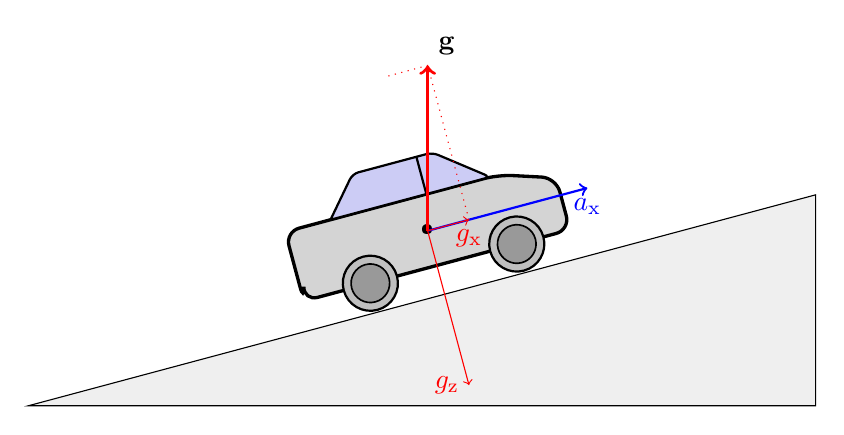
\begin{tikzpicture}[scale=1]
    % Define/Calc ramp parameters
    % Ramp length
    \def\rl{10};
    % Ramp angle [deg]
    \def\ra{15};
    % Ramp height
    \def\rh{{tan(\ra)*\rl}};

    % RAMP
    % Define the points
    \coordinate (A) at (0,0);
    \coordinate (B) at ($(A) + (\rl,0)$);
    \coordinate (C) at ($(B) + (0,\rh)$);
    % Draw and fill ramp
    \filldraw[draw=black, fill=lightgray!25] (A) -- (B) -- (C) -- cycle;

    % CAR
    % Tilt whole car
    \begin{scope}[scale=0.7, xshift=\rl*0.5 cm, yshift=1.9 cm, rotate=\ra]
        % Car height
        \def\ch{2}
        % Car length
        \def\cl{5}
        % Car body height
        \def\bh{\ch*0.65}
        % Roof length
        \def\rl{\cl*0.6}
        % Roof height
        \def\rh{\ch*0.35}
        % Car tilt angle
        \def\ct{6}

        % Anchor point is southwest
        \coordinate (b) at (0,0);
        % Offset to roof and wheels
        \coordinate (r) at ($(b) +(\cl*0.17,\ch*0.65)$);
        \coordinate (w) at ($(b) + (\cl*0.25,0)$);
        % Body
        \draw[black, fill=black!17, rounded corners=1.2ex, very thick]
        (b) -- ++(0,\bh) -- ++(\cl*1/5,0) --  ++(\cl*3/5,0) -- ++(\cl*1/5,-\bh*0.25)
        -- ++(0, -\bh*0.75) -- (b) -- cycle;
        % Roof
        \draw[very thick, rounded corners=0.5ex, fill=black!20!blue!20!white,thick]
        (r) -- ++(0.2*\rl,\rh) -- ++(0.5*\rl,0) -- ++(0.3*\rl,-\rh) -- (r);
        \draw[thick] (r)++(\rl*0.6,0) -- ++(0,\rh);

        % % Car middle point
        \coordinate (m) at (\cl*0.5, \bh*0.5);
        \node at (m) {\textbullet};
        % Wheels
        \draw[draw=black,fill=gray!50,thick] (w) circle (.5);
        \draw[draw=black,fill=gray!50,thick] (w) ++(\cl*0.55,0) circle (.5);
        % Inner wheels
        \draw[draw=black,fill=gray!80,semithick] (w) circle (.35);
        \draw[draw=black,fill=gray!80,semithick] (w) ++(\cl*0.55,0) circle (.35);

        % Draw car acceleration
        \draw[blue, thick, ->] (m) -- ++(3,0) node[anchor=north]{$a_\mathrm{x}$};
        % Gravity vectors
        % Length of g vector
        \def\gl{3}
        % Length of g vector components
        \def\gxl{{\gl*sin(\ra)}}
        \def\gzl{{\gl*cos(\ra)}}
        % Draw vectors
        \draw[red, ->, very thick, rotate=-\ra] (m) -- ++(0,\gl) node[anchor=south west, black](g_end){$\mathbf{g}$};
        \draw[red, thin, ->] (m) -- ++(\gxl,0) node[anchor=north]{$g_\mathrm{x}$};
        \draw[red, thin, ->] (m) -- ++(0,-\gzl) node[anchor=east]{$g_\mathrm{z}$};
        \draw[red, dotted] ($(m)+(\gxl,0)$) -- ++(0,\gzl) -- ++(-\gxl,0);
    \end{scope}
\end{tikzpicture}
\end{document}
	\caption{The prevailing accelerations when a car is accelerating on a ramp.}
	\label{fig:tikz_car_gravity}
\end{figure}
\subsubsection{Gyroscope}
\iimprov{Find good source and use it as a guide}
The gyroscope measures the angular velocity, which must be integrated with respect to time, to get a rotation angle.
The angular velocity the rate of change of an angle and is defined as
\begin{equation}
	% \boldsymbol{\omega}  = \frac{\Delta\theta}{\Delta t}
	\boldsymbol{\omega}  =  \dv{\boldsymbol{\theta}}{t}.
\end{equation}
Assuming that the measurements of the gyroscope are continuous in time, the current angle $\boldsymbol{\theta}(t)$ at time $T$ can be computed with the integral
\begin{equation}
	\boldsymbol{\theta}(t) = \boldsymbol{\theta}_0 + \int_0^T \boldsymbol{\omega}(t)\dd{t}
\end{equation}
with $\boldsymbol{\theta}_0$ being the initial angle.\\
In practice, however, the \gls{imu} provides samples at discrete times $k$ and $k-1$.
Assuming that the signal remains constant during the time $\Delta t$ between the two samples, the integral can be numerical approximated.
An error will be introduced by the approximation, but it will be small if the sample rate is sufficiently high.
Different techniques exist, using the ? method the new angle after a change between two samples can be calculated with
\begin{equation}
	\boldsymbol{\theta}_k = \boldsymbol{\theta}_\mathrm{k - 1} + \boldsymbol{\omega}_k\Delta t.
\end{equation}
Similarly, the angle based on multiple consecutive measurements can be calculated by the sum of all previous measurements
\begin{equation}
	\label{eq:ang_from_gyro}
	\boldsymbol{\theta}_k = \boldsymbol{\theta}_0 + \sum_{i = 1}^k \boldsymbol{\omega}_i \Delta t
\end{equation}
with $\boldsymbol{\theta}_0$ being the initial angle at the start of the measurement, which must be known beforehand.\\
To get the pitch angle $\theta_\mathrm{gyr}$, only the measurements along the y-axis are of interest (see \cref{fig:tikz_car_frames}).
The pitch angle at time $k$ is given by
\begin{equation}
	\theta_\mathrm{k, gyr} = \theta_{0, \mathrm{gyr} } + \sum_{i = 1}^{k} \boldsymbol{\omega}_\mathrm{i, y} \Delta t.
\end{equation}
Disadvantages of using only the angular velocity are that the estimations are not reliable over a long period of time.
The random walk introduced by integrating white noise or a constant bias causes the estimation to drift away from the true value.


\subsubsection{Complementary filter}
The complementary uses both the linear acceleration and angular velocity measurements and combines them using sensor fusion, such that the good properties of each sensor are used to reduce the poor properties of the other.
The angle estimation obtained from the linear acceleration measurements is reliable in the long-term, but is quite noisy.
The estimation from the angular velocity measurements on the other hand provide good short-term accuracy, but should not be used for longer estimations due to drift.\\
These properties can be interpreted in the frequency domain.
The error from the accelerometer data is subject to high frequency noise, whereas the estimation error from the gyroscope is mostly due to low frequency noise \cite{2007Colton}.
To minimize the error of the linear acceleration estimate, a \gls{lpf} should be used.
A \gls{lpf} passes all signals with frequency lower than a certain cut-off frequency $f_0$ and attenuates signals with a frequency above $f_0$.
In contrast, a \gls{hpf} should be used on the estimate of the gyroscope.
A \gls{hpf} works exactly opposite to a \gls{lpf}.
It blocks signals with a frequency below $f_0$ while allowing signals over this frequency to pass through \cite{Lyons1996}. A block diagram of the complementary filter is shown in \cref{fig:tikz_complementary_filter}.\\
\begin{figure}[htb]
	\centering
	\documentclass[12pt]{standalone}
\usepackage{tikz}

\usetikzlibrary{calc, positioning}

\begin{document}
% Define styles
\tikzstyle{block} = [draw, minimum width=2cm, minimum height=1.2cm]

\begin{tikzpicture}
    % Sum shape
    \node[draw, circle, minimum size=0.6cm] (sum) at (0,0){+};

    % LP-Filter block
    \node [block, above left=0.1cm and 1cm of sum] (lpf) {Low-Pass Filter};
    % HP-Filter block
    \node [block, below left=0.1cm and 1cm of sum] (hpf) {High-Pass Filter};
    % Integrator block
    \node [draw, minimum height=1.2cm, left=1.5cm of hpf] (int) {$\int$};

    % Connect blocks with sum
    \draw[-stealth] (lpf.east) -| (sum.north);
    \draw[-stealth] (hpf.east) -| (sum.south);

    % Input signals
    \node [left=3cm of lpf] (start_acc){};
    \node [below=1.7cm of start_acc] (start_gyr){};
    \draw[stealth-] (lpf.west) -- (start_acc) node[left]{$\theta_\mathrm{acc}$};
    \draw[stealth-] (int.west) -- (start_gyr) node[left]{$\dot{\theta}_\mathrm{gyr}$};
    \draw[-stealth] (int.east) -- (hpf.west) node[midway, above]{$\theta_\mathrm{gyr}$};
    \draw[-stealth] (sum.east) -- ++(1,0) node[right]{$\hat{\theta}$};
\end{tikzpicture}
\end{document}
	\caption{Block diagram of the complementary filter}
	\label{fig:tikz_complementary_filter}
\end{figure}
The angle estimation obtained from the linear acceleration (\cref{eq:ang_from_acc}) will be referred to as $\theta_\mathrm{acc}$, the angle estimation from the gyroscope estimation as $\theta_\mathrm{gyr}$ and the fused estimation of the complementary filter will be denoted as $\hat{\theta}$.
As seen in \cref{eq:ang_from_gyro}, $\theta_\mathrm{gyr}$ is calculated by integrating the angular velocity $\omega_\mathrm{gyr} $ measured by the gyroscope.
The Laplace transformation can be used to transform the angles from the time domain to the frequency domain.
The angles $\theta_\mathrm{acc}$, $\theta_\mathrm{gyr}$ and $\hat{\theta}$ will be denoted as $\Theta_\mathrm{acc}(s)$, $\Theta_\mathrm{gyr}(s)$ and $\hat{\Theta}(s)$ in the frequency domain, the gyroscope measurements $\omega_\mathrm{gyr} $ as $\Omega_\mathrm{gyr} (s)$.
The complimentary filter estimate is computed by
\begin{align}
	\label{eq:compl_filter_laplace}
	\hat{\Theta}(s) & = G_\mathrm{low}(s)\Theta_\mathrm{acc}(s) + (1 - G_\mathrm{low}(s))\Theta_\mathrm{gyr}(s) \nonumber   \\
	                & = G_\mathrm{low}(s)\Theta_\mathrm{acc}(s) + (1 - G_\mathrm{low}(s))\frac{1}{s}\Omega_\mathrm{gyr} (s)
\end{align}
where $G_\mathrm{low}(s)$ is the transfer function of a \gls{lpf} and $1-G_\mathrm{low}(s) = G_\mathrm{high}(s)$ the of a \gls{hpf} \cite{Kok2017}.
The sum of $G_\mathrm{low}(s)$ and $1-G_\mathrm{low}(s)$ is equal to one, which means that the cut-off frequency of both filters must be the same.
The transfer functions are defined as
\begin{equation}
	\label{eq:lpf}
	G_\mathrm{low} (s) = \frac{1}{1 + \alpha s}
\end{equation}
for the \gls{lpf} and
\begin{equation}
	\label{eq:hpf}
	G_\mathrm{high} (s) = \frac{\alpha s}{1 + \alpha s}
\end{equation}
for the \gls{hpf}, when using a first-order filter.
$\alpha$ is the filter coefficient and is depended on the cut-off frequency in the following way
\begin{equation}
	\alpha
	= \frac{\tau}{\tau + T}
	% = \frac{1}{w_0}
	= \frac{1}{2\pi f_0}
	\label{eq:filter_f0}
\end{equation}
with $\tau$ being the time constant of the filter and $T$ being the sample period.
Inserting \cref{eq:lpf} and \cref{eq:hpf} in \cref{eq:compl_filter_laplace} and using inverse Laplace transformation as well as Euler backward discretization, the complementary filter can be written in discrete time as
\begin{equation}
	\hat{\theta}_k = \gamma\left(\hat{\theta}_{k - 1} + T \omega_{k, \mathrm{gyr}}\right) + (1 - \gamma) \theta_{k, \mathrm{acc}},
\end{equation}
with
\begin{equation}
	\label{eq:filter_gain}
	\gamma = \frac{\alpha}{\alpha + T} \in [0,1]
\end{equation}
being the filter gain.
The choice of the parameter $\alpha$ (and hence $\gamma$) determines, how much each of the two measurements should be trusted.
Selecting a small $\alpha$ ($\gamma$ close to zero) results in a high cut-off frequency.
The estimation then mostly uses the accelerometer data.
Contrary, a high value of $\alpha$ leads to a $\gamma$ close to one and low cut-off frequency, where the gyroscope estimation is trusted more \cite{1997Baerveldt}.\\
% A decrease of $\alpha$ leads to a smoother signal, but at the cost of adding some additional time delay.
Selecting the right filter coefficient is a known problem and is usually solved by calculating an initial guess followed by fine-tuning by hand to get the desired result.
One option to get an initial guess is by measuring the drift of the gyroscope and selecting the filter coefficient accordingly.
The time $T_\mathrm{free}$ where the drift of the angle estimation from the gyroscope is negligible, is inversely proportional to the cut-off frequency $f_0 = \frac{1}{T_\mathrm{free}}$.
E.g. if the drift from the gyroscope is only negligible for \SI{10}{\second} then the cut-off frequency should be chosen at $f_0 = \frac{1}{\SI{10}{\second}} = \SI{0.1}{\hertz}$ or higher.
The filter gain can then be calculated using \cref{eq:filter_f0} and \cref{eq:filter_gain}.
Using the previous example and assuming a sample frequency of \SI{100}{\hertz}, the filter gain would then be $\gamma = 0.9938$.
For the experiment a cut-off frequency of $f_0=?$ was chosen, resulting in a filter coefficient of $\alpha = ?$ and a filter gain of $\gamma = ?$.

\subsubsection{Gravity method}
\label{subsubsec:gravity_method}
% \subsubsubsection{Car acceleration from odometer data}
% \label{subsubsec:acc_from_odom}
As described in \cref{ssec:linear_acceleration_only}, the linear acceleration measurements can be used to determine the pitch angle.
But the estimation is only valid under the condition, that there are no accelerations other than the acceleration due to gravity.
This condition is not necessarily true when the car is driving, during which the car can accelerate or brake.
To get the correct estimation, the car's acceleration must be subtracted from the measurement.
\paragraph{Car acceleration from odometer data}\mbox{}\\
Using the wheel speed measurements the velocity of the vehicle can be calculated.
Because the wheel speed sensors only deliver the speed of each wheel, a model has to be used to estimate the velocity of the car.
Because setting one wheel speed measurement equal to the velocity of the car would lead to a wrong estimation, since during turns the left and right wheels travel at different speeds, the wheel on the inner side of the turn travels slower, than the outer wheel.
A simple yet sufficiently accurate model to calculate the car velocity from the wheel speeds is the linear single track model \cite{Mitschke2014}.
In this model both wheels on one axis are replaced with one wheel in the middle.
The linear assumption holds true for low lateral accelerations (up to \SI{4}{\metre\per\second}), which will not be surpassed in the experiments.
Using the assumptions from above, the car velocity $v_\mathrm{car}(t)$ can be calculated by
\begin{align}
	\alpha(t)         & = \frac{v_\mathrm{rl}(t) - v_\mathrm{rr}(t)}{d}                  \\
	\gamma(t)         & = \frac{\alpha(t)}{f_\mathrm{odom}}                              \\
	v_\mathrm{car}(t) & = \frac{v_\mathrm{rl}(t) + v_\mathrm{rr}(t)}{2}\cdot\cos(\gamma)
	\label{eq:v_car}
\end{align}
with $v_\mathrm{rl} \text{ and } v_\mathrm{rr}$ being the wheel speeds of the rear right and rear left wheel respectively, $d$ the track width and $\gamma$ is the yaw angle of the car, which can be calculated from the steering wheel angle.\\
To calculate the acceleration of the vehicle, the first derivative of the velocity must be taken, using
\begin{equation}
	a_\mathrm{car}(t) = \dv{t}v_\mathrm{car}(t).
\end{equation}
But because all measurements are discrete, numerical differentiation is necessary, it can be approximated using the backward difference
\begin{equation}
	a_\mathrm{k, car} = \frac{v_\mathrm{k, car} - v_\mathrm{k - 1, car}}{T}
\end{equation}
with $T$ being the step size, which is equal to the rate of the sensor.\\
Because the from the wheel speed sensors calculated velocity is discrete in time, quantized and not free of noise, a simple derivation would amplify the noise.
Hence, the measurements must first be filtered.
\itodo{Investigate other filters such as savitzky-golay once and for all}
A very simple solution is to use a moving average filter, which is a simple average of the last $N$ measurements.
The finite difference of the approximation can then be calculated.
\paragraph{Gravity method}\mbox{}\\
The prevailing accelerations during a positive acceleration can be seen in \cref{fig:tikz_car_gravity}.
When the car brakes, the direction of $\vb{a}_\mathrm{x}$ inverts.
The car pitch angle calculation is the same as in \cref{eq:ang_from_acc}, just that now the car acceleration $\vb{a}_\mathrm{at}$ is taken into account.
\begin{equation}
	\label{eq:ang_from_acc_gravity}
	\alpha = \arcsin\left(\frac{\vb{a}_\mathrm{x} - \vb{a}_\mathrm{at}}{\norm{\vb{g}}}\right)
	= \arcsin\left(\frac{\vb{a}_\mathrm{x} - \dv{t}v_\mathrm{at} }{\norm{\vb{g}}}\right)
\end{equation}
with $\vb{a}_\mathrm{x}$ being the acceleration measured by the x-axis of the \gls{imu} and $\norm{\vb{g}}$ being the magnitude of the overall measured acceleration.
It is important the both the \gls{imu} and odometer measurements are synchronized in time, otherwise a change in acceleration leads to a wrong estimation.

\subsection{Ramp detection}
\label{ssec:ramp_detection_imu}
\iimprov{This section needs improvement}
In the previous section different methods to estimate the pitch angle of the car were presented.
Assuming that the car is accelerating moderately and other factors which might engage the suspension, such as road vibrations or ? are minimal, the estimated pitch angle can be assumed to be close to the road grade.
Using the estimated road grade, it can be determined whether the car is on a ramp.
If the absolute number of the road grade surpasses a certain threshold, the part is classified as a ramp, otherwise it is classified as a normal road.\\
Because the angle of a ramp is not constant, but increases and decreases at the beginning and end respectively, only the average angle can be estimated.
The average angle of the ramp is calculated by \todo{sth}.
The length of the ramp can be calculated by integrating the velocity of the car over time.
The velocity can be calculated in two different ways.
Using the wheel speed measurements (\cref{eq:v_car}), or by integrating the accelerometer measurements along the x-axis.
The problem when using the accelerometer data is that also other accelerations than the one caused by the car are measured.
If the car is on a ramp, the acceleration due to gravity is measured as well.
But using \cref{eq:ang_from_acc} and transforming it to
\begin{equation}
	\hat{a}_\mathrm{car} = \vb{a}_\mathrm{x} - \sin(\theta) \norm{\vb{g}}
\end{equation}
the acceleration due to gravity can be removed from the measurements, under the assumption that the estimated car pitch angle is close to the true value.
The length $l$ of the ramp can then be calculated by first integrating the acceleration with respect tot time to get the velocity
\begin{equation}
	\hat{v}_\mathrm{i, car} = \hat{a}_\mathrm{0, car} + \sum_{i = 1}^k \hat{a}_\mathrm{i, car} \Delta t                         \\
\end{equation}
and then integrating the velocity to get the length
\begin{equation}
	l = \sum_{i = 1}^k v_\mathrm{i, car} \Delta t                         \\
\end{equation}
where the velocity $v_\mathrm{i, car}$ is the velocity at the start of the ramp and $v_\mathrm{k, car}$ is the velocity at the end of the ramp.


\section{\glsentryshort{lidar} only}
\label{sec:methods_lidar}
\itodo{Maybe brief overview of section/algorithm}
\subsection{Calibration}
\label{ssec:calibration_lidar}
Same as for the \gls{imu}, a transformation from the \gls{lidar} frame to the car frame is necessary.
The calibration is very similar to that of the \gls{imu}.
At first both z-axes will be aligned.
This is achieved by detecting the ground plane in the point cloud and finding the transform, such that the normal vector of the plane aligns with the z-axis of the car (the plane gets projected onto the xy-plane of the car frame).
This results in the correct pitch and roll angle.
The yaw angle can not be easily determined and is assumed to be equal to zero, but can also be measured by hand and given as parameter.\\
For the ground plane detection \gls{ransac} \cite{Fischler1981} is used.\\
\gls{ransac} is a non-deterministic algorithm to remove outliers and is often used in computer vision.
\gls{ransac} can also be used for plane segmentation in 3D point clouds.
Consider a point cloud with $n$ points, where point $i$ has the coordinates $x_i, y_i, z_i$.
In a first step, three random points from the point cloud are selected.
Three, because this is the minimum number of points necessary to create a plane.
Now the parameters $a, b, c, d$ of the plane equation
\begin{equation}
	ax + by + cz + d = 0
\end{equation}
can be calculated.
Then for every other point the deviation $r$ from the proposed plane can be calculated by
\begin{equation}
	r = \frac{ax_i + by_i + cz_i + d}{\sqrt{a^2 + b^2 + c^2}}
\end{equation}
and is then summed up.
If the distance is within a certain threshold, the point counts as an inlier.
After iterating through the whole point cloud, the number of inlier points and their coordinates are stored.
This process is then repeated until the maximal number of iterations are reached.
The plane with the greatest number of inliers is then selected.\\
Then the normal vector of the plane, which can be conducted from the plane equation as follows
\begin{equation}
	\vb{n} = \left(\begin{array}{lll} a & b & c \end{array}\right)^{\intercal}
\end{equation}
is projected onto the z-axis of the car.
The necessary rotation is then applied to the detected plane.
Now that a plane has been found it must be ensured, that it really is the ground plane.
Typically, either the ceiling, ground or a side wall gets detected with \gls{ransac}.
The greater the plane is (or the more points lie inside a plane), the more likely is the detection of the plane.
Due to the mounting and \gls{fov} of the \gls{lidar}, the ceiling usually does have the most points and is thus detected in the first iteration.\\
An accidental ceiling detection can be prevented by looking at the average z-values of the detected plane.
Because the \gls{lidar} is mounted on the roof of the car, the z-values of the detected plane must be negative.
If they are positive, the ceiling has been detected.
Furthermore, it is known, that the calculated roll angle should be minimal.
If that is not the case, most likely a side wall has been detected.
If either condition has not been fulfilled, the detected plane does get removed from the point cloud and using \gls{ransac} a new ground plane estimation is made and validated.
This process gets repeated until both conditions are fulfilled.
The yaw angle and the x- and y-translation from the \gls{lidar} to the centered front of the car
must be entered manually, but the pitch and roll angle and the distance from the \gls{lidar} to the ground are used from the calibration.


\subsection{Algorithm}
\iimprov{Maybe divide into subsubsections, e.g. ramp detection, ramp props etc}
\subsubsection{Point cloud preprocessing}
\begin{figure}[htb]
	\centering
	\documentclass[11pt]{standalone}
\usepackage{tikz}
\usetikzlibrary{shapes.geometric, arrows}

% Define shapes
\tikzstyle{startstop} = [rectangle, rounded corners, minimum width=3cm, minimum height=.7cm,text centered, draw=black, fill=red!30]
\tikzstyle{io} = [trapezium, trapezium left angle=80, trapezium right angle=100, minimum width=2cm, minimum height=.7cm, text centered, draw=black, fill=blue!30]
\tikzstyle{process} = [rectangle, minimum width=3cm, minimum height=.7cm, text centered, text width=3.5cm, draw=black, fill=orange!30]
\tikzstyle{decision} = [diamond, aspect=3, minimum width=3cm, minimum height=.7cm, text centered, draw=black, fill=green!30]
\tikzstyle{arrow} = [thick,->,>=stealth]

\begin{document}
\begin{tikzpicture}[node distance=1.2cm]
    % \node (start) [startstop] {Start};
    % \node (raw) [io, below of=start] {Raw \acrshort{lidar} point cloud};
    \node (calibration) [startstop] {Calibration};
    \node (raw) [io, below of=calibration] {Raw LiDAR point cloud};
    \node (transform) [process, below of=raw] {Transform};
    \node (passthrough) [process, below of=transform] {Passthrough filter};
    \node (downsample) [process, below of=passthrough] {Downsample};
    \node (is_enough_points) [decision, below of=downsample, yshift=-0.5cm] {Points \& Iterations left?};
    \node (ransac) [process, below of=is_enough_points, yshift=-0.5cm] {RANSAC};
    \node (is_ramp) [decision, below of=ransac, yshift=-0.3cm] {Angle \& width?};
    \node (reduce) [process, right of=is_ramp, xshift=4cm] {Remove plane};
    \node (rotmat) [io, below of=is_ramp, yshift=-0.3cm] {Ramp properties};
    \node (skip) [startstop, left of=rotmat, xshift=-3cm] {Skip};
    % \node (end) [startstop, below of=rotmat] {Stop};


    % Connect the nodes
    % \draw [arrow] (start) -- (raw);
    \draw [arrow] (calibration) -- (raw);
    \draw [arrow] (raw) -- (transform);
    \draw [arrow] (transform) -- (passthrough);
    \draw [arrow] (passthrough) -- (downsample);
    \draw [arrow] (downsample) -- (is_enough_points);
    \draw [arrow] (is_enough_points) -- node[anchor=west] {yes} (ransac);
    \draw [arrow] (is_enough_points) -| node[anchor=east] {no} (skip);
    \draw [arrow] (ransac) -- (is_ramp);
    \draw [arrow] (is_ramp) -- node[anchor=east] {yes} (rotmat);
    \draw [arrow] (is_ramp) -- node[anchor=north] {no} (reduce);
    \draw [arrow] (reduce) |- (is_enough_points);
    % \draw [arrow] (rotmat) -- (end);
\end{tikzpicture}
\end{document}
	\caption{Flow chart of the ramp detection algorithm using the \acrshort{lidar} sensor.}
	\label{fig:flowchart_lidar}
\end{figure}
Because the raw \gls{lidar} data is too big to allow for real time processing, preprocessing is necessary.
It consists of a passthrough filter to remove unwanted points (e.g. behind the car) and a voxel grid filter to downsample the point cloud.
Before the passthrough filter can be applied, the point cloud must be transformed to the car frame.
The in the previous section described calibration algorithm is performed once at the start and its returned rotation is then applied to every new measurement.\\
The passthrough filter then removes all the points which lie outside the specified x, y and z limits.
Because the car drives forward, only points in front of the car are of interest.
Furthermore, the points further away than a certain threshold are neglected, because the resolution and accuracy of the measurements of the \gls{lidar} decreases with increasing distance.
The ceiling points are removed by limiting the points in z-direction.
The exact values used for the passthrough filter can be seen along the other parameters in \cref{tab:lidar_params}.\\
The next step in reducing the point cloud size is the voxel grid filter \cite{Vosselman2004}.
The point cloud is converted into a 3D grid consisting of small cubes called voxels.
Each cube can contain multiple points or none, the size of the voxels (also known as leaf size) determines the resolution.
All the points inside a cube are then reduced to their most centroid point.
If the cube does not contain any points, it is neglected.
\subsubsection{Ramp detection}
Now that the point cloud size is reduced greatly the actual ramp detection can be performed with sufficient performance.
The \gls{ransac} algorithm usually detects the following types of planes: ceiling, ground, side wall or the desired ramp.
\gls{ransac} is applied iteratively until a plane of type ramp has been found.
If a plane of different type has been found, it gets removed and the \gls{ransac} algorithm is applied again.
To prevent an infinite loop, the algorithm will exit after either a certain number of iterations has been performed, or if after the removal of a plane not enough points are left in the point cloud.
For the implementation of the \gls{ransac} algorithm and the voxel grid filter the PCL library \cite{Rusu2011} has been used.\\
The accidental detection of the ceiling was already prevented during the passthrough filter step, where the ceiling points have been removed from the point cloud.
Wrong detections of the ground plane or side walls can be prevented by requiring the angle to be in a certain range.

\subsubsection{Ramp properties}
\label{sssec:ramp_properties}
\iimprov{This section needs imporovement}
Beside the angle, the width of the plane (y-range) is being calculated and compared to the parameters, to make sure that the plane is a drivable ramp for cars and not e.g. a small ramp for wheelchairs \todo{no idea if wheel chair ramps are common in parking garages?}.
The distance to the ramp is estimated by taking the $n$ nearest points of the ramp plane and calculating their mean.
If a ramp has been detected, the estimated angle and distance from the car front to the beginning of the ramp are returned.\\
A visual representation of the algorithm is depicted in \cref{fig:flowchart_lidar}.
\iimprov{Explain flow chart better}
\isug{What happens with stairs?}
\itodo{Add down ramp detection}
\iimprov{Add some more algo parameters to table (full one in appendix)}
\begin{table}[H]
	\centering
	\caption{Used parameters for lidar algo}
	\label{tab:lidar_params}
	\begin{tabular}[t]{lc}
		\toprule
		\textbf{parameter} & \textbf{value}          \\
		\midrule
		\textbf{Passthrough filter}                  \\
		x                  & \SIrange{0}{30}{\metre} \\
		y                  & \SIrange{-2}{2}{\metre} \\
		z                  & \SIrange{-1}{2}{\metre} \\
		\midrule
		\textbf{Voxel filter}                        \\
		leaf size          & \SI{0.1}{\metre}        \\
		\midrule
		\textbf{\gls{ransac}}                        \\
		max iter           & 100                     \\
		distance threshold & \SI{0.11}{\metre}       \\
		normal distance w  & 0.01                    \\
		\midrule
		\textbf{rd}                                  \\
		angle              & \SIrange{3}{9}{\degree} \\
		width              & \SIrange{2}{6}{\metre}  \\
		$o$                & 4                       \\
		\bottomrule
	\end{tabular}
\end{table}%



\section{Camera only}
In this section an approach using the images captured by the camera to detect a ramp is presented.
At first, the choice of a deep learning network as the method of choice to solve this task is explained.
In the next section the generation of the dataset used for the training is described.
And finally the training of the network and the choice of the different hyperparameters is discussed.

\subsection{Approach}
Different techniques exist, more classic methods like edge detection and thresholding or more sophisticated methods like machine learning.
While less complex methods like edge detection and thresholding might work, they require a well lit environment with a high contrast between different textures, which is not the case in the parking garage.
Furthermore, the features need to be chosen manually, and the algorithm would most probably only work in a very limited certain environment.\\
That is why a deep learning method has been chosen instead.
It is more robust and can easily be adapted to other environments.
The choice of the network depends on the problem.
Different approaches such as object detection, instance or semantic segmentation are available.
For this project, the instance semantic approach was chosen.
While the object detection approach requires the least computational effort, it only provides a bounding box around the object.
Both segmentation approaches on the other hand create a mask around the object, allowing for a more accurate localization of the object.
For the specific task of detecting ramps in parking garages the semantic segmentation would probably be enough since most times only one ramp will be visible, in which case the semantic and instance segmentation will be the same.
But the instance segmentation approach is more general and can be adapted more easily to support also the detection of other objects.
That is why the mask \gls{rcnn} neural network architecture is used in this thesis.
It allows for instance segmentation, which means that multiple objects of the same class can be detected as distinct objects.
\itodo{Semantic segmentation would not be any worse than instance segmentation}
While for this task only one class is used (ramp) and most times only one object will be visible, the network can be easily expanded to support multiple classes and is already supporting the detection of multiple ramps at once.
Furthermore, it is well documented, and different implementations are already available for use.\\
For this thesis the open-source \texttt{Detectron2}~\footnote{\url{https://github.com/facebookresearch/detectron2}} \cite{Wu2019} library developed by Facebook is chosen as the framework.
It is widely used and also provides a number of pretrained networks, which can be used for transfer learning.
Transfer learning is the process of training a new model on top of an existing one.
This provides multiple advantages over training a new model from scratch, such as a great reduction of the training time and hence also the use of resources, a better accuracy and reducing the risk of overfitting.\\
A model trained on the \gls{coco} dataset \cite{Lin2014} is used as the basis for the training of the network.
\gls{coco} is a large-scale dataset consisting of more than \num{200000} labeled images with various annotations (e.g. bounding boxes, segmentation masks, image captions) of 80 different object categories (e.g. car, chair, dog, person, train).
It is often used to benchmark neural network algorithms and to compare their performance.\\
Since no class of type ramp already exists in the \gls{coco} dataset, an own dataset has to be created.
\iimprov{Write here already about point cloud extraction?}


\subsection{Dataset}
While several datasets specifically for the task of autonomous driving already exist, no dataset with ramps as a class could be found.
That is why an own dataset had to be created, by taking pictures of a ramp and labeling them by hand.
To reduce the workload, for the creation of the dataset only straight ramps as shown are considered.
The three different ramps shown in FIGURE are used for the training.
\missingfigure{Three ramps}
Multiple recordings of each ramp were made from different distances and angles.
The images were taken from a video with a frame rate of 30, but since the car approached the ramp with a low speed of \SI{5}{\kilo\metre\per\hour}, the difference between two frames is very small.
Since many pictures of the more or less same scenery do not provide any extra information, while increasing the training time and the potential of overfitting, only every 30th image (one every second) was used.
80? different were collected in the end.
Since the training of the network is based on supervised learning, the images have to be labelled manually.
For this task the tool \texttt{labelme}~\footnote{\url{https://github.com/wkentaro/labelme}} \cite{Wada2018} is used.
Each ramp is labelled using a polygon consisting of four points, placed at the corners of the ramp.
The \texttt{labelme} tool creates an annotation containing the coordinate of each point, which had to be converted to \gls{coco} format, which also calculates a bounding box of the polygon.
Data augmentation \cite{Shorten2019}.
\missingfigure{Some labeled examples of different ramps and angles}

\subsection{Training}
Since the size of the dataset is not very great, the training of the network is challenging, because it increases the risk of overfitting.
To alleviate the problem, data augmentation is used in addition to the previously mentioned transfer learning.
Data augmentation provides a good alternative to when the collection of more data is not feasible or possible.
It increases the size of the dataset by adding slightly modified versions of the original images.
Common transformations are horizontal or vertical flipping of the image, cropping, adding noise, blur or changing the brightness and contrast of the image.
The library \texttt{imgaug}~\footnote{\url{https://github.com/aleju/imgaug}} \cite{Jung2018} is used for this task.
In addition to editing the image, it automatically adapts the annotation according to the new position of the label, e.g. when flipping the image.
The following augmentations techniques are used to increase the dataset: horizontal flipping of the image (with a probability of 50\%), changing the brightness by \SIrange{-50}{50}{\percent}, changing the contrast by \SIrange{-20}{10}{\percent}, adding motion blur with a kernel size of 3 and adding Gaussian blur with a kernel with a sigma in the range of \SIrange{0}{1}{}.
All the added changes are also common occurrences in the real world, which should help to improve the accuracy of the network in other environments.
One augmentation is performed on each image which is then added to the dataset.
To evaluate the performance of the network, the dataset has to be split into a training and a validation set.
The split is done before the data augmentation to ensure, that the training set does not contain any only slightly modified versions of the images used in the validation set.
Due to the small size of the dataset, 80\% of the dataset is used for the training and 20\% for the validation set.\\
The accuracy of the network depends on the correct choice of multiple hyperparameters.
Since the dataset is small and thus the training using transfer learning does not take very long, different hyperparameter configurations could be tested to find the best one.
One of the most important parameters is the learning rate.
It is often in the range of \SIrange{0.0}{1.0}{} and describes how fast the weights of the network are updated.
Is the learning rate too low, the training of the network takes a longer time and might not converge to find a solution, whereas if the learning rate is too high, a suboptimal solution might be found.
The learning rate is often initially set to a high value and then slowly reduced, which helps both optimization and generalization.
The speed of the decay of the learning rate can be based on many things, such as the number of steps in the training, the time, or it can be reduced exponentially.
In this thesis, an approach where the learning rate is decayed after every $n$ steps is used.
Another parameter, specifically for the mask \gls{rcnn} neural network architecture, is the number of \gls{roi} proposals.
As described in \cref{sssec:rcnn}, the image is divided into a grid of \glspl{roi}.
The number of \gls{roi} proposals determines how many of those \glspl{roi} are taken into account for the calculation.
It can be chosen lower than the size of the grid to accelerate the training.
The final parameter which will be varied is the number of epochs.
It describes how often the network is trained on the entire dataset, a higher number of epochs means a longer training time, but usually also a better performance, except if it is chosen to high, in which case it can lead to overfitting.

\subsection{Point cloud extraction}
The ZED 2i stereo camera used in this thesis also generates point cloud.
More information about the camera can be found in \cref{ssec:camera}.
\itodo{Only bounding box atm, how to use mask?}
The point cloud can be projected on the camera image.
For the projection the rotation vector and translation from the point cloud frame to the camera frame is necessary, as well as the intrinsic camera matrix $A$.
Using the \texttt{projectPoints} function of the \texttt{opencv} library \cite{Bradski2000}, the point cloud is projected onto the camera image.
Using the predicted bounding box, all the projected points outside the box are removed.
The points are then transformed back into the 3D space.
By applying the \gls{ransac} algorithms outliers are removed and a model of the ramp is created.
Different properties of the ramp can now be calculated, similarly as described in \cref{ramp_properties}.
